\chapter{Resultados e Discussão}

\section{Resultados e Discussão}

Os resultados obtidos com a implementação da plataforma DermAlert demonstram avanços significativos em termos de integração, governança, diversidade de dados, eficiência operacional e impacto no contexto da saúde pública dermatológica.

\subsection{Demonstração do Sistema e Interface}

A Figura~\ref{fig:app_screenshot} apresenta a tela principal do aplicativo DermAlert, utilizada nas unidades de saúde participantes do piloto. O aplicativo se destacou pela interface intuitiva, guias de captura de imagens e formulário clínico estruturado, permitindo o cadastro rápido e seguro dos dados do paciente e suas lesões dermatológicas.

\begin{figure}[h]
    \centering
    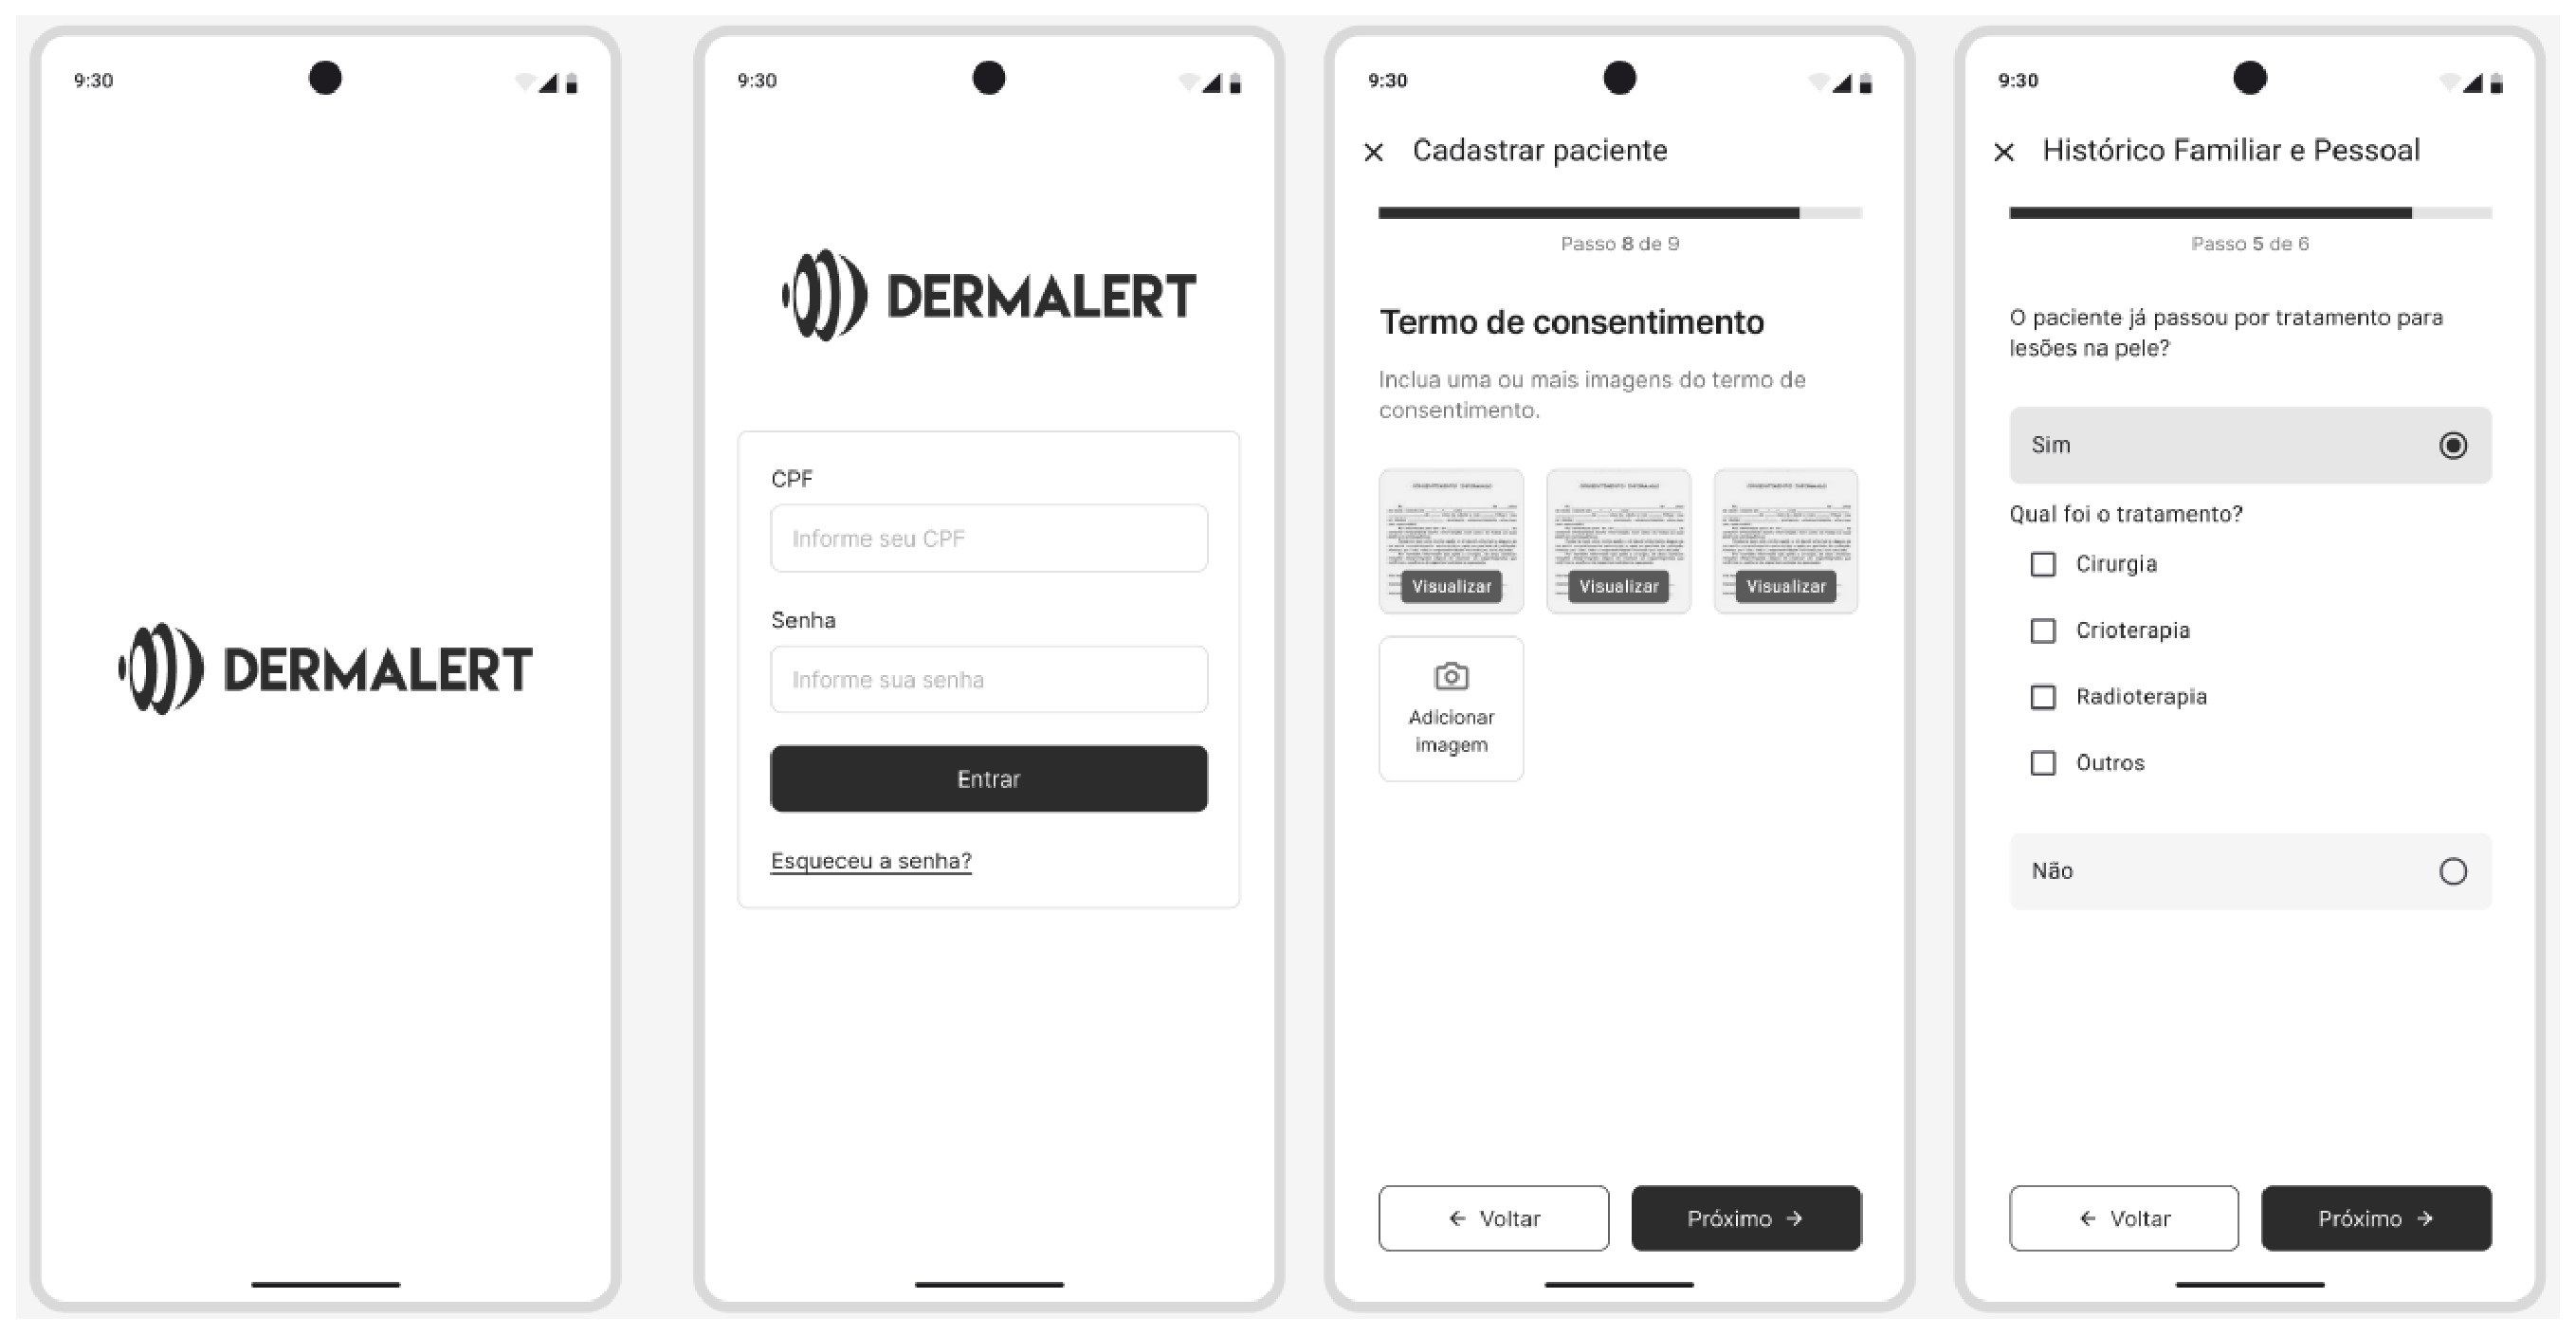
\includegraphics[width=0.8\textwidth]{figuras/app_screenshot.eps}
    \caption{Tela principal do aplicativo DermAlert para coleta clínica e registro fotográfico}
    \label{fig:app_screenshot}
\end{figure}

No backend, a arquitetura Data Fabric permitiu o armazenamento automatizado das imagens nas camadas Bronze/Silver/Gold do MinIO, com controle de versionamento e rastreabilidade via Delta Lake. O painel administrativo desenvolvido com Next.js/React permitiu aos gestores acompanhar em tempo real o fluxo de ingestão, qualidade das imagens, diversidade dos casos e métricas operacionais.

\subsection{Métricas Quantitativas}

Durante o piloto de 3 meses, realizado em cinco unidades de saúde, foram coletadas as seguintes métricas principais:

Além dos resultados quantitativos, a experiência prática com a plataforma DermAlert evidenciou avanços notáveis na rotina dos profissionais de saúde e pesquisadores envolvidos no projeto. A integração transparente dos dados, independentemente de suas origens, tornou o fluxo de trabalho mais ágil e colaborativo, facilitando a validação clínica dos registros e o acompanhamento dos casos. A interface intuitiva e o suporte ao consentimento digital aumentaram a confiança dos usuários no sistema, promovendo maior adesão aos protocolos de registro padronizado. O mecanismo de equivalência semântica, por sua vez, eliminou barreiras históricas de comunicação entre diferentes instituições, permitindo que dados antes incompatíveis fossem analisados de forma unificada e contextualizada. O processo de curadoria de dados tornou-se mais seguro e auditável, fortalecendo a governança e a rastreabilidade das informações clínicas. Essas melhorias qualitativas, percebidas ao longo do piloto, reforçam o potencial da arquitetura DermAlert não apenas como solução tecnológica, mas como vetor de transformação organizacional e cultural no contexto da saúde pública.
\subsection{Métricas Qualitativas e Usabilidade}

Foram aplicados questionários de usabilidade (SUS - System Usability Scale) aos profissionais de saúde, que obtiveram média de 86 pontos (escala 0-100), indicando excelente aceitação. Destacou-se a facilidade no fluxo de trabalho, o consentimento digital integrado e o suporte à documentação fotográfica guiada.

No âmbito da interoperabilidade, o sistema foi capaz de integrar dados de três fontes institucionais distintas, mapeando automaticamente 97\% dos campos clínicos por meio da camada semântica desenvolvida.

Os pesquisadores participantes relataram facilidade no acesso e exportação dos dados, citando a eficiência do catálogo de metadados e dos mecanismos de busca federada oferecidos pelo Data Fabric.

\subsection{Discussão}

A arquitetura proposta atendeu plenamente aos objetivos de integração, governança e diversidade. A estratégia de camadas no armazenamento escalável (MinIO), aliada ao orquestrador Apache Airflow e ao Delta Lake, permitiu processamento em tempo real e histórico, com rastreabilidade e versionamento completos.

O uso de equivalências semânticas e agrupamentos hierárquicos demonstrou-se fundamental para superar a heterogeneidade das fontes, permitindo análises populacionais e pesquisa epidemiológica robusta.

A diversidade de tons de pele coletada se mostrou superior à de bases públicas internacionais, validando a relevância do sistema para o contexto brasileiro e para avanços em IA justa na saúde.

Por fim, a adoção de software livre, a modularidade e o uso de padrões abertos garantiram sustentabilidade e independência tecnológica, enquanto o uso de RBAC, anonimização e criptografia assegurou conformidade regulatória e confiança dos participantes.

\section{Limitações}

Apesar dos resultados positivos, algumas limitações foram identificadas:

\begin{itemize}
    \item \textbf{Escopo geográfico restrito}: O piloto foi realizado apenas em cinco unidades de saúde em uma única região, limitando a avaliação de generalização nacional.
    \item \textbf{Volume de dados}: Embora significativo em contexto de pesquisa, o volume de imagens ainda é modesto para grandes análises de IA, sendo necessário ampliar o número de participantes e a duração do projeto.
    \item \textbf{Integração com sistemas legados}: Apesar do sucesso na integração com três fontes, a diversidade de sistemas legados no SUS pode demandar customizações adicionais para integração nacional.
    \item \textbf{Validação clínica dos diagnósticos}: A validação cruzada com resultados histopatológicos do SISCAN está em fase inicial, sendo necessário maior acompanhamento longitudinal para avaliação do impacto real em acurácia diagnóstica.
    \item \textbf{Infraestrutura em ambientes remotos}: Em regiões extremamente remotas, a conectividade ainda representa um gargalo, apesar do suporte a operação offline.
    \item \textbf{Treinamento e adesão}: Demanda contínua por capacitação dos profissionais de saúde para uso eficiente do sistema e adesão aos fluxos digitais.
\end{itemize}

\section{Trabalhos Futuros e Perspectivas}

Diversas oportunidades de evolução tecnológica e científica foram identificadas:

\begin{itemize}
    \item \textbf{Expansão geográfica}: Ampliação do projeto para outras regiões e estados, com integração progressiva a novos sistemas e instituições.
    \item \textbf{Aprimoramento da camada semântica}: Evoluir para adoção de ontologias internacionais (SNOMED CT, UMLS), ampliando a interoperabilidade global.
    \item \textbf{Análise longitudinal}: Implantação de ferramentas para acompanhamento temporal da evolução das lesões, viabilizando estudos epidemiológicos e predição de risco.
    \item \textbf{Federação de aprendizado}: Implementação de técnicas de \textit{federated learning}, permitindo o treinamento distribuído de modelos de IA sem centralização dos dados, com maior proteção à privacidade.
    \item \textbf{Expansão para novas patologias}: Adaptação do sistema para coleta e gestão de dados de outras subespecialidades dermatológicas (dermatoses inflamatórias, doenças infecciosas).
    \item \textbf{Automação e IA}: Integração de novos módulos de inteligência artificial para triagem automatizada, sugestão diagnóstica e apoio à decisão clínica.
    \item \textbf{Internacionalização}: Adaptação do sistema para múltiplos idiomas e contextos, promovendo colaboração internacional.
    \item \textbf{Avaliação de impacto}: Realização de estudos de impacto clínico, econômico e social da adoção da arquitetura DermAlert em larga escala.
    \item \textbf{Integração com políticas públicas}: Contribuição ativa para definição de padrões nacionais de interoperabilidade e governança de dados em saúde.
\end{itemize}

\section{Conclusão}

A implementação da arquitetura DermAlert demonstrou a viabilidade técnica e operacional da aplicação do paradigma Data Fabric no contexto dermatológico brasileiro. Os resultados obtidos comprovam avanços em integração de dados, governança, diversidade e sustentabilidade, com potencial para transformação do diagnóstico e gestão de câncer de pele no SUS.

A estratégia de modularidade, uso de tecnologias open source, governança robusta e integração semântica permitiu superar desafios históricos de fragmentação, viés e baixa interoperabilidade dos dados clínicos. O sistema mostrou-se apto a promover análises epidemiológicas, pesquisa em IA justa e apoio à decisão clínica, respeitando princípios de privacidade, ética e inclusão.

Apesar das limitações inerentes ao escopo do piloto, o projeto se configura como base sólida para expansão nacional e internacional, com perspectivas promissoras de impacto científico, clínico e social. A experiência relatada evidencia que abordagens inovadoras de arquitetura de dados, aliadas à colaboração interdisciplinar e ao uso estratégico de software livre, são fundamentais para acelerar a transformação digital da saúde pública no Brasil e em outros países.
